\documentclass[conference]{IEEEtran}
\IEEEoverridecommandlockouts

\usepackage{cite}
\usepackage{amsmath,amssymb,amsfonts}
\usepackage{algorithm, algorithmic}
\usepackage{graphicx}
\usepackage{textcomp}
\usepackage{xcolor}
\def\BibTeX{{\rm B\kern-.05em{\sc i\kern-.025em b}\kern-.08em
    T\kern-.1667em\lower.7ex\hbox{E}\kern-.125emX}}

% Custom packages
\usepackage[capitalise]{cleveref}
\usepackage{tikz}
\usepackage{pgfplots}
\usepackage{nicefrac}
\usepackage{siunitx}
\usepackage{booktabs}
\usepackage{multirow}
\sisetup{mode = match}
\usepackage[T1]{fontenc}

% TikZ libraries
\usetikzlibrary{shapes.geometric, arrows.meta, positioning, calc, patterns, fit, backgrounds, matrix}
\pgfplotsset{compat=1.17}

% Define colors
\definecolor{matlabBlue}{RGB}{0,114,189}
\definecolor{matlabOrange}{RGB}{217,83,25}
\definecolor{matlabYellow}{RGB}{237,177,32}
\definecolor{matlabPurple}{RGB}{126,47,142}
\definecolor{matlabGreen}{RGB}{119,172,48}
\definecolor{lstmColor}{RGB}{70,130,180}
\definecolor{attentionColor}{RGB}{255,165,0}
\definecolor{fcColor}{RGB}{60,179,113}

\begin{document}
\title{Attention-Enhanced LSTM Networks for Steering Torque Prediction in Electric Power Steering Systems}

\author{\IEEEauthorblockN{Tianze Liang}
\IEEEauthorblockA{\textit{School of Computation, Information and Technology} \\
\textit{Technical University of Munich (TUM)}\\
Munich, Germany \\
tianze.liang@tum.de}
\and
\IEEEauthorblockN{Robert Wille}
\IEEEauthorblockA{\textit{Chair for Design Automation} \\
\textit{Technical University of Munich (TUM)}\\
Munich, Germany \\
robert.wille@tum.de}
}

\maketitle

\begin{abstract}
Electric Power Steering (EPS) systems are safety-critical components in modern vehicles that require precise steering torque prediction for reliable operation within complex electrical and electronic (E/E) architectures.
This paper presents a data-driven approach combining Long Short-Term Memory (LSTM) networks with attention mechanisms to predict steering torque from vehicle dynamics data.
We systematically compare three attention mechanisms: Simple Attention, Additive Attention (Bahdanau), and Scaled Dot-Product Attention (Luong).
Experimental results on real-world driving data from the commaSteeringControl dataset demonstrate that the LSTM model with Simple Attention achieves the highest prediction accuracy of \qty{89.71}{\percent}, outperforming the baseline LSTM (\qty{84.66}{\percent}) by approximately \qty{5}{\percent}.
Furthermore, we analyze the trade-off between model complexity and prediction accuracy, showing that simpler model structures achieve comparable performance with significantly reduced training time (\qty{79}{\percent} reduction).
The proposed approach provides an efficient solution for steering torque prediction suitable for resource-constrained embedded systems in vehicles.
\end{abstract}

\begin{IEEEkeywords}
LSTM, attention mechanism, electric power steering, steering torque prediction, time series forecasting, deep learning, vehicle dynamics
\end{IEEEkeywords}

%%%
% INTRODUCTION
%%%
\section{Introduction}
\label{sec:introduction}

Electric Power Steering (EPS) systems have become essential components in modern vehicles, providing steering assistance while reducing driver effort and enabling advanced driver assistance features~\cite{isah2019electric}.
As automotive electrical and electronic (E/E) architectures evolve toward greater complexity with increasing integration of Advanced Driver Assistance Systems (ADAS), EPS systems face significant challenges in ensuring reliable and precise steering control~\cite{salih2020computation}.

Traditional physics-based approaches for EPS control rely on mathematical models derived from vehicle dynamics~\cite{govender2016modelling}.
However, these approaches struggle to capture the nonlinear relationships inherent in real-world driving scenarios, such as friction effects, variable tire stiffness, and external disturbances~\cite{zheng2023research}.
Data-driven approaches offer a promising alternative by learning complex patterns directly from sensor measurements without explicit physical modeling~\cite{vanwijk2022data}.

Predicting steering torque is crucial for several reasons: (1) it enables proactive power management in the E/E architecture by anticipating high-demand scenarios, (2) it provides predictive reference values for safety redundancy systems, and (3) it improves system responsiveness by reducing real-time computational delays.
Despite these benefits, existing research primarily focuses on steering angle prediction~\cite{xing2020driver}, % TODO: Replace reference - Xing et al. 2019 is about driver activity recognition, NOT steering angle prediction
while steering torque prediction using modern deep learning techniques with attention mechanisms remains largely unexplored.

Long Short-Term Memory (LSTM) networks have demonstrated excellent performance in time series prediction tasks due to their ability to capture both short-term and long-term temporal dependencies~\cite{hochreiter1997long}.
Attention mechanisms, originally developed for machine translation~\cite{bahdanau2016neural}, can enhance LSTM networks by dynamically weighting the importance of different time steps in the input sequence~\cite{vaswani2017attention}.

This paper makes the following contributions:
\begin{itemize}
    \item We present a systematic comparison of three attention mechanisms (Simple, Additive, and Scaled Dot-Product) for steering torque prediction in EPS systems.
    \item We demonstrate that Simple Attention achieves the highest prediction accuracy (\qty{89.71}{\percent}) while maintaining low computational complexity suitable for embedded systems.
    \item We provide a comprehensive analysis of the trade-off between model complexity and prediction accuracy, showing that simpler models can achieve comparable performance with significantly reduced training time.
    \item We validate our approach using real-world driving data from the commaSteeringControl dataset, demonstrating practical applicability.
\end{itemize}

The remainder of this paper is organized as follows: \cref{sec:related_work} reviews related work. \cref{sec:methodology} describes the proposed methodology. \cref{sec:experimental_setup} presents the experimental setup. \cref{sec:results} discusses the results, and \cref{sec:conclusion} concludes the paper.

%%%
% RELATED WORK
%%%
\section{Related Work}
\label{sec:related_work}

\subsection{Physics-Based Approaches for EPS Control}

Traditional EPS control systems rely on physics-based modeling and classical control algorithms.
Govender et al.~\cite{govender2016pid} evaluated advanced PID structures including two-degree-of-freedom PID and cascade PID for front steering angle control, finding that these controllers struggle with nonlinear systems and are sensitive to parameter variations.
Subsequently, state-space methods such as pole placement and linear quadratic control were proposed to improve performance~\cite{govender2016pid}.

To address nonlinearities, Marouf et al.~\cite{marouf2011control} introduced Sliding Mode Control (SMC) for EPS, demonstrating robust performance in simulations.
Lee et al.~\cite{lee2018robust} proposed Adaptive Sliding Mode Control (ASMC) to ensure robustness against uncertainties.
However, SMC-based approaches often suffer from control chattering, causing oscillations in output torque~\cite{shtessel2014sliding}.
Zheng and Wei~\cite{zheng2023research} presented an Active Disturbance Rejection Control (ADRC) strategy to filter noise and estimate disturbances effectively.

While physics-based approaches offer interpretability, they require accurate system models and struggle with external disturbances that vary in real driving scenarios.

\subsection{Data-Driven Approaches for Vehicle Dynamics}

Data-driven methods learn patterns between inputs and outputs without requiring explicit physical models.
Van Wijk et al.~\cite{vanwijk2022data} proposed a Hidden Markov Model-based approach combined with Gaussian Mixture Regression for driver steering torque estimation, demonstrating effective learning of nonlinear relationships.
Zhao et al.~\cite{zhao2022modeling} developed steering feedback torque prediction for steer-by-wire systems using Artificial Neural Networks (ANNs) and Gaussian Process Regression.

LSTM networks have been widely applied in time series forecasting tasks.
Wang et al.~\cite{wang2016financial} demonstrated the effectiveness of recurrent neural networks for financial time series prediction.
Attention mechanisms have been integrated with LSTM for various applications, including power load forecasting~\cite{wan2023short} and traffic prediction~\cite{li2023ultra}.
Recent work by Wen and Li~\cite{wen2023time} showed that LSTM-Attention models outperform standard LSTM for general time series prediction.

However, the application of attention-enhanced LSTM networks specifically for EPS steering torque prediction has not been systematically investigated, representing a research gap that this paper addresses.

%%%
% METHODOLOGY
%%%
\section{Methodology}
\label{sec:methodology}

\subsection{Problem Formulation}

The steering torque prediction task is formulated as a multivariate time series forecasting problem.
Given historical measurements of vehicle dynamics features, the goal is to predict the normalized steering torque at a future time step.

Let $\mathbf{X} = (\mathbf{x}_1, \mathbf{x}_2, \ldots, \mathbf{x}_L)$ denote a sequence of input features, where $\mathbf{x}_t \in \mathbb{R}^N$ represents the $N$-dimensional feature vector at time step $t$, and $L$ is the sliding window length.
The objective is to predict the target value $y_{L+1}$ at time step $L+1$.

The input features selected based on vehicle dynamics equations include:
\begin{itemize}
    \item Vehicle speed $v_{\text{ego}}$ (m/s)
    \item Longitudinal acceleration $a_{\text{ego}}$ (m/s\textsuperscript{2})
    \item Steering wheel angle $\theta_{\text{sw}}$ (degrees)
    \item Road roll angle $\phi$ (rad)
    \item Lateral acceleration $a_{\text{lat}}$ (m/s\textsuperscript{2})
\end{itemize}

These features are derived from the steering torque equation of the upper steering shaft~\cite{peng2013simulation}:
\begin{equation}
    T_{\text{sw}} = T_s + B_{\text{sw}}\dot{\theta}_{\text{sw}} + J_{\text{sw}}\ddot{\theta}_{\text{sw}}
    \label{eq:torque}
\end{equation}
where $T_{\text{sw}}$ is the steering wheel torque, $T_s$ is the steering shaft torque, $B_{\text{sw}}$ is the damping coefficient, and $J_{\text{sw}}$ is the steering wheel inertia.

\subsection{LSTM-Based Foundation Model}

The baseline model architecture consists of stacked LSTM layers followed by a fully connected layer, as illustrated in \cref{fig:architecture}.
Each LSTM cell processes a time step in the input sequence, maintaining both a cell state $\mathbf{c}_t$ for long-term memory and a hidden state $\mathbf{h}_t$ for short-term dependencies.

The LSTM cell operations, including the forget gate introduced by Gers et al.~\cite{gers2000learning}, are defined as:
\begin{align}
    \mathbf{f}_t &= \sigma(\mathbf{W}_f[\mathbf{h}_{t-1}, \mathbf{x}_t] + \mathbf{b}_f) \label{eq:forget}\\
    \mathbf{i}_t &= \sigma(\mathbf{W}_i[\mathbf{h}_{t-1}, \mathbf{x}_t] + \mathbf{b}_i) \label{eq:input}\\
    \tilde{\mathbf{c}}_t &= \tanh(\mathbf{W}_c[\mathbf{h}_{t-1}, \mathbf{x}_t] + \mathbf{b}_c) \label{eq:candidate}\\
    \mathbf{c}_t &= \mathbf{f}_t \odot \mathbf{c}_{t-1} + \mathbf{i}_t \odot \tilde{\mathbf{c}}_t \label{eq:cell}\\
    \mathbf{o}_t &= \sigma(\mathbf{W}_o[\mathbf{h}_{t-1}, \mathbf{x}_t] + \mathbf{b}_o) \label{eq:output_gate}\\
    \mathbf{h}_t &= \mathbf{o}_t \odot \tanh(\mathbf{c}_t) \label{eq:hidden}
\end{align}
where $\mathbf{f}_t$, $\mathbf{i}_t$, and $\mathbf{o}_t$ are the forget, input, and output gates, respectively, $\sigma$ denotes the sigmoid function, and $\odot$ represents element-wise multiplication.

%%% Figure: Model Architecture
\begin{figure}[t]
    \centering
    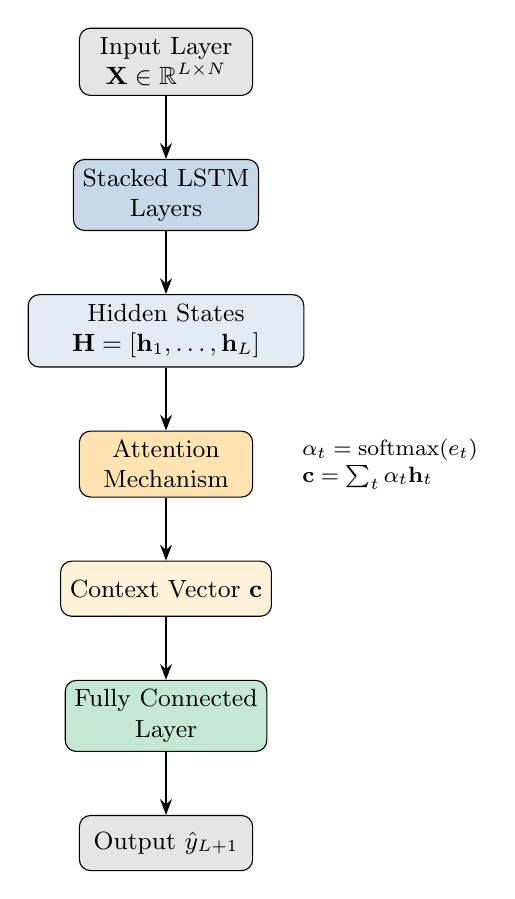
\begin{tikzpicture}[
        node distance=0.8cm,
        box/.style={rectangle, draw, rounded corners, minimum width=2.2cm, minimum height=0.7cm, align=center, font=\small},
        arrow/.style={-{Stealth[length=2mm]}, thick}
    ]
        % Input Layer
        \node[box, fill=gray!20] (input) {Input Layer\\$\mathbf{X} \in \mathbb{R}^{L \times N}$};
        
        % LSTM Layers
        \node[box, fill=lstmColor!30, below=of input] (lstm) {Stacked LSTM\\Layers};
        
        % Hidden States
        \node[box, fill=lstmColor!15, below=of lstm, minimum width=3.5cm] (hidden) {Hidden States\\$\mathbf{H} = [\mathbf{h}_1, \ldots, \mathbf{h}_L]$};
        
        % Attention
        \node[box, fill=attentionColor!30, below=of hidden] (attention) {Attention\\Mechanism};
        
        % Context Vector
        \node[box, fill=attentionColor!15, below=of attention] (context) {Context Vector $\mathbf{c}$};
        
        % FC Layer
        \node[box, fill=fcColor!30, below=of context] (fc) {Fully Connected\\Layer};
        
        % Output
        \node[box, fill=gray!20, below=of fc] (output) {Output $\hat{y}_{L+1}$};
        
        % Arrows
        \draw[arrow] (input) -- (lstm);
        \draw[arrow] (lstm) -- (hidden);
        \draw[arrow] (hidden) -- (attention);
        \draw[arrow] (attention) -- (context);
        \draw[arrow] (context) -- (fc);
        \draw[arrow] (fc) -- (output);
        
        % Side annotation
        \node[right=0.5cm of attention, align=left, font=\footnotesize] {$\alpha_t = \text{softmax}(e_t)$\\$\mathbf{c} = \sum_t \alpha_t \mathbf{h}_t$};
    \end{tikzpicture}
    \caption{Architecture of the proposed LSTM-Attention model for steering torque prediction.}
    \label{fig:architecture}
\end{figure}

\subsection{Attention Mechanisms}

To enhance the model's ability to focus on relevant time steps, we integrate attention mechanisms between the LSTM layers and the fully connected layer.
We investigate three attention mechanisms with different computational approaches.

\subsubsection{Simple Attention}

The Simple Attention mechanism independently evaluates the importance of each time step using a single linear transformation:
\begin{align}
    e_t &= \mathbf{W}_e \mathbf{h}_t + b_e \label{eq:linear_score}\\
    \alpha_t &= \frac{\exp(e_t)}{\sum_{k=1}^{L} \exp(e_k)} \label{eq:linear_weight}\\
    \mathbf{c} &= \sum_{t=1}^{L} \alpha_t \mathbf{h}_t \label{eq:linear_context}
\end{align}
where $\mathbf{W}_e \in \mathbb{R}^{1 \times d_h}$ and $b_e \in \mathbb{R}$ are learnable parameters, $d_h$ is the hidden state dimension, $\alpha_t$ are the attention weights, and $\mathbf{c}$ is the context vector.

This mechanism introduces minimal additional parameters ($d_h + 1$) while enabling the model to weight different time steps according to their relevance for prediction.

\subsubsection{Additive Attention (Bahdanau)}

Additive Attention, proposed by Bahdanau et al.~\cite{bahdanau2016neural}, computes pairwise attention scores using a feed-forward network:
\begin{align}
    e_{ij} &= \mathbf{v}_a^T \tanh(\mathbf{W}_a \mathbf{h}_i + \mathbf{U}_a \mathbf{h}_j) \label{eq:additive_score}\\
    \alpha_{ij} &= \frac{\exp(e_{ij})}{\sum_{k=1}^{L} \exp(e_{ik})} \label{eq:additive_weight}\\
    \mathbf{c}_i &= \sum_{j=1}^{L} \alpha_{ij} \mathbf{h}_j \label{eq:additive_context}
\end{align}
where $\mathbf{W}_a, \mathbf{U}_a \in \mathbb{R}^{d_a \times d_h}$ and $\mathbf{v}_a \in \mathbb{R}^{d_a}$ are learnable parameters, and $d_a$ is the attention dimension.

This mechanism captures correlations between different time steps, allowing each position to incorporate information from all other positions.
The total number of parameters is $2d_h d_a + d_a$.

\subsubsection{Scaled Dot-Product Attention (Luong)}

Scaled Dot-Product Attention computes attention scores through dot products between hidden states~\cite{vaswani2017attention}:
\begin{align}
    e_{ij} &= \frac{\mathbf{h}_i^T \mathbf{h}_j}{\sqrt{d_h}} \label{eq:dotprod_score}\\
    \alpha_{ij} &= \frac{\exp(e_{ij})}{\sum_{k=1}^{L} \exp(e_{ik})} \label{eq:dotprod_weight}\\
    \mathbf{c}_i &= \sum_{j=1}^{L} \alpha_{ij} \mathbf{h}_j \label{eq:dotprod_context}
\end{align}

The scaling factor $\sqrt{d_h}$ prevents the dot products from becoming too large for high-dimensional vectors, which would push the softmax function into regions with extremely small gradients~\cite{vaswani2017attention}.
This mechanism introduces no additional learnable parameters.

%%% Figure: Attention Mechanisms Comparison
\begin{figure}[t]
    \centering
    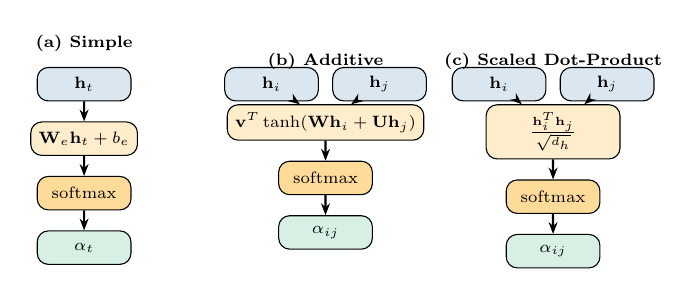
\begin{tikzpicture}[
        node distance=0.4cm,
        smallbox/.style={rectangle, draw, rounded corners, minimum width=1.4cm, minimum height=0.5cm, align=center, font=\scriptsize},
        arrow/.style={-{Stealth[length=1.5mm]}, thick},
        scale=0.85, transform shape
    ]
        % Simple Attention
        \begin{scope}[local bounding box=linear]
            \node[smallbox, fill=lstmColor!20] (h1) {$\mathbf{h}_t$};
            \node[smallbox, fill=attentionColor!20, below=0.3cm of h1] (linear) {$\mathbf{W}_e \mathbf{h}_t + b_e$};
            \node[smallbox, fill=attentionColor!40, below=0.3cm of linear] (soft1) {softmax};
            \node[smallbox, fill=fcColor!20, below=0.3cm of soft1] (alpha1) {$\alpha_t$};
            \draw[arrow] (h1) -- (linear);
            \draw[arrow] (linear) -- (soft1);
            \draw[arrow] (soft1) -- (alpha1);
            \node[above=0.1cm of h1, font=\scriptsize\bfseries] {(a) Simple};
        \end{scope}
        
        % Additive Attention
        \begin{scope}[xshift=2.8cm, local bounding box=additive]
            \node[smallbox, fill=lstmColor!20] (h2i) {$\mathbf{h}_i$};
            \node[smallbox, fill=lstmColor!20, right=0.2cm of h2i] (h2j) {$\mathbf{h}_j$};
            \node[smallbox, fill=attentionColor!20, below=0.3cm of $(h2i)!0.5!(h2j)$, minimum width=2.2cm] (add) {$\mathbf{v}^T \tanh(\mathbf{W}\mathbf{h}_i + \mathbf{U}\mathbf{h}_j)$};
            \node[smallbox, fill=attentionColor!40, below=0.3cm of add] (soft2) {softmax};
            \node[smallbox, fill=fcColor!20, below=0.3cm of soft2] (alpha2) {$\alpha_{ij}$};
            \draw[arrow] (h2i) -- (add);
            \draw[arrow] (h2j) -- (add);
            \draw[arrow] (add) -- (soft2);
            \draw[arrow] (soft2) -- (alpha2);
            \node[above=0.1cm of $(h2i)!0.5!(h2j)$, font=\scriptsize\bfseries] {(b) Additive};
        \end{scope}
        
        % Scaled Dot-Product Attention
        \begin{scope}[xshift=6.2cm, local bounding box=dotprod]
            \node[smallbox, fill=lstmColor!20] (h3i) {$\mathbf{h}_i$};
            \node[smallbox, fill=lstmColor!20, right=0.2cm of h3i] (h3j) {$\mathbf{h}_j$};
            \node[smallbox, fill=attentionColor!20, below=0.3cm of $(h3i)!0.5!(h3j)$, minimum width=2cm] (dot) {$\frac{\mathbf{h}_i^T \mathbf{h}_j}{\sqrt{d_h}}$};
            \node[smallbox, fill=attentionColor!40, below=0.3cm of dot] (soft3) {softmax};
            \node[smallbox, fill=fcColor!20, below=0.3cm of soft3] (alpha3) {$\alpha_{ij}$};
            \draw[arrow] (h3i) -- (dot);
            \draw[arrow] (h3j) -- (dot);
            \draw[arrow] (dot) -- (soft3);
            \draw[arrow] (soft3) -- (alpha3);
            \node[above=0.1cm of $(h3i)!0.5!(h3j)$, font=\scriptsize\bfseries] {(c) Scaled Dot-Product};
        \end{scope}
    \end{tikzpicture}
    \caption{Comparison of the three investigated attention mechanisms: (a) Simple Attention evaluates each time step independently, (b) Additive Attention uses a feed-forward network, and (c) Scaled Dot-Product Attention computes dot products.}
    \label{fig:attention_mechanisms}
\end{figure}

%%%
% EXPERIMENTAL SETUP
%%%
\section{Experimental Setup}
\label{sec:experimental_setup}

\subsection{Dataset}

We use the commaSteeringControl dataset~\cite{commasteeringcontrol}, which contains vehicle steering measurements collected with the openpilot ADAS system~\cite{openpilot}.
The dataset includes sensor data from various vehicle models; for this study, we select data from the 2020 Hyundai Sonata equipped with a Column-type Electric Power Steering (C-EPS) system.

Due to time and computational resource limitations, data from the first 5001 CSV files of the 2020 Hyundai Sonata were selected, each containing approximately 60 seconds of driving data recorded at 10~Hz sampling frequency.
We filter the data to include only segments where the openpilot system is fully engaged (latActive = True) and the driver is not intervening (steeringPressed = False), ensuring consistent autonomous steering behavior.

The target variable is the normalized, rate-limited steering torque (steerFiltered), ranging from $-1$ to $1$.
This normalization enables generalization across different vehicle models with varying torque ranges.

\subsection{Data Preprocessing}

Data preprocessing involves the following steps:
\begin{enumerate}
    \item Each CSV file is assigned a unique sequence ID to maintain temporal continuity.
    \item Missing and duplicate values are removed.
    \item Features are selected based on vehicle dynamics equations (\cref{eq:torque}).
    \item A sliding window technique with window size $L=50$ (5 seconds at 10~Hz) is applied to create training samples.
\end{enumerate}

The sliding window moves forward by one time step for each sample, creating overlapping sequences that capture the temporal evolution of vehicle dynamics.

\subsection{Implementation Details}

All models are implemented using the PyTorch Lightning framework (version 2.5.0) and trained on an NVIDIA GeForce RTX 3070 Ti GPU with 8~GB VRAM.

The dataset is split into training (\qty{70}{\percent}), validation (\qty{20}{\percent}), and test (\qty{10}{\percent}) sets.
Training samples are shuffled to improve generalization, while validation and test samples maintain temporal order.

We use Mean Squared Error (MSE) as the loss function:
\begin{equation}
    \mathcal{L}_{\text{MSE}} = \frac{1}{n}\sum_{i=1}^{n}(y_i - \hat{y}_i)^2
    \label{eq:mse}
\end{equation}

The Adam optimizer~\cite{kingma2015adam} is used with a learning rate determined through Bayesian hyperparameter optimization using the Optuna library~\cite{akiba2019optuna} with Tree-structured Parzen Estimator (TPE).
Early stopping with patience of 5 epochs prevents overfitting.

\subsection{Evaluation Metrics}

We evaluate model performance using the following metrics:

\textbf{Accuracy:} The percentage of predictions with absolute error below a threshold $\epsilon = 0.05$:
\begin{equation}
    \text{Accuracy} = \frac{1}{n}\sum_{i=1}^{n}\mathbb{I}(|y_i - \hat{y}_i| \leq \epsilon)
    \label{eq:accuracy}
\end{equation}

\textbf{Root Mean Squared Error (RMSE):}
\begin{equation}
    \text{RMSE} = \sqrt{\frac{1}{n}\sum_{i=1}^{n}(y_i - \hat{y}_i)^2}
    \label{eq:rmse}
\end{equation}

\textbf{Time Cost Ratio (TCR):} The ratio of training time for a complex model to reach the same accuracy as a simpler model:
\begin{equation}
    \text{TCR} = \frac{T_{\text{complex}}}{T_{\text{simple}}}
    \label{eq:tcr}
\end{equation}

\textbf{Learning Efficiency (LE):} The rate of accuracy improvement per hour:
\begin{equation}
    \text{LE} = \frac{\text{Acc}_{t_2} - \text{Acc}_{t_1}}{t_2 - t_1}
    \label{eq:le}
\end{equation}

%%%
% RESULTS AND DISCUSSION
%%%
\section{Results and Discussion}
\label{sec:results}

\subsection{Baseline LSTM Performance}

The baseline LSTM model with hidden size 64 and 3 layers achieves \qty{84.66}{\percent} accuracy and RMSE of 0.00116 on the test set.
The validation accuracy increases rapidly during early training and gradually converges, reaching a maximum of \qty{85.06}{\percent}.

Increasing model complexity (hidden size 128, 5 layers) yields only marginal improvement to \qty{86.75}{\percent}, despite a 7-fold increase in model parameters (from 0.339~MB to 2.391~MB).
This limited improvement indicates that the baseline LSTM architecture cannot fully utilize additional capacity, motivating the integration of attention mechanisms.

\subsection{Impact of Attention Mechanisms}

\cref{tab:attention_comparison} presents the performance comparison of LSTM models with different attention mechanisms.
All attention-enhanced models outperform the baseline LSTM, demonstrating the effectiveness of attention for steering torque prediction.

%%% Table: Attention Comparison
\begin{table}[t]
    \centering
    \caption{Performance Comparison of LSTM Models with Different Attention Mechanisms}
    \label{tab:attention_comparison}
    \begin{tabular}{lcc}
        \toprule
        \textbf{Model} & \textbf{Accuracy (\%)} & \textbf{RMSE} \\
        \midrule
        Baseline LSTM & 84.66 & 0.00116 \\
        LSTM + Simple Attention & \textbf{89.71} & \textbf{0.00098} \\
        LSTM + Additive Attention & 88.82 & 0.00101 \\
        LSTM + Scaled Dot-Product Attention & 88.65 & 0.00101 \\
        \bottomrule
    \end{tabular}
\end{table}

The LSTM with Simple Attention achieves the highest accuracy (\qty{89.71}{\percent}) and lowest RMSE (0.00098).
Notably, this simpler attention mechanism outperforms both Additive and Scaled Dot-Product Attention, which capture pairwise time step correlations.

This result suggests that for steering torque prediction, independently evaluating the importance of each time step is more effective than modeling complex inter-time-step dependencies.
The steering torque at a given moment is primarily influenced by recent vehicle dynamics rather than long-range correlations.

%%% Figure: Training Curves
\begin{figure}[t]
    \centering
    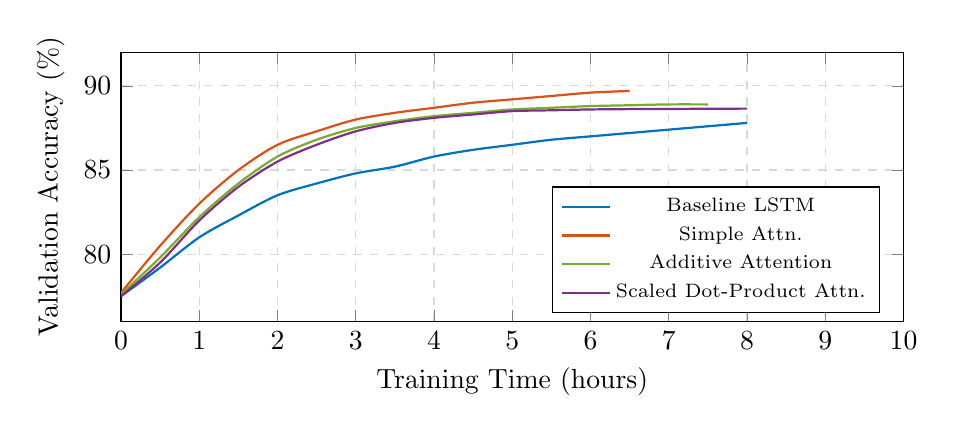
\begin{tikzpicture}
        \begin{axis}[
            width=0.95\columnwidth,
            height=5cm,
            xlabel={Training Time (hours)},
            ylabel={Validation Accuracy (\%)},
            xmin=0, xmax=10,
            ymin=76, ymax=92,
            legend pos=south east,
            legend style={font=\scriptsize},
            grid=major,
            grid style={dashed, gray!30},
        ]
        % Baseline LSTM
        \addplot[color=matlabBlue, thick, smooth] coordinates {
            (0,77.5) (0.5,79.2) (1,81.0) (1.5,82.3) (2,83.5) (2.5,84.2) (3,84.8) (3.5,85.2) (4,85.8) (4.5,86.2) (5,86.5) (5.5,86.8) (6,87.0) (6.5,87.2) (7,87.4) (7.5,87.6) (8,87.8)
        };
        \addlegendentry{Baseline LSTM}
        
        % Simple Attention
        \addplot[color=matlabOrange, thick, smooth] coordinates {
            (0,77.7) (0.5,80.5) (1,83.0) (1.5,85.0) (2,86.5) (2.5,87.3) (3,88.0) (3.5,88.4) (4,88.7) (4.5,89.0) (5,89.2) (5.5,89.4) (6,89.6) (6.5,89.7)
        };
        \addlegendentry{Simple Attn.}
        
        % Additive Attention
        \addplot[color=matlabGreen, thick, smooth] coordinates {
            (0,77.6) (0.5,79.8) (1,82.2) (1.5,84.2) (2,85.8) (2.5,86.8) (3,87.5) (3.5,87.9) (4,88.2) (4.5,88.4) (5,88.6) (5.5,88.7) (6,88.8) (6.5,88.85) (7,88.9) (7.5,88.9)
        };
        \addlegendentry{Additive Attention}
        
        % Scaled Dot-Product Attention
        \addplot[color=matlabPurple, thick, smooth] coordinates {
            (0,77.5) (0.5,79.5) (1,82.0) (1.5,84.0) (2,85.5) (2.5,86.5) (3,87.3) (3.5,87.8) (4,88.1) (4.5,88.3) (5,88.5) (5.5,88.55) (6,88.6) (6.5,88.62) (7,88.63) (7.5,88.64) (8,88.65)
        };
        \addlegendentry{Scaled Dot-Product Attn.}
        
        \end{axis}
    \end{tikzpicture}
    \caption{Validation accuracy over training time for different models. The LSTM with Simple Attention converges faster and achieves higher accuracy.}
    \label{fig:training_curves}
\end{figure}

\cref{fig:training_curves} shows the validation accuracy trajectories during training.
The LSTM with Simple Attention not only achieves the highest final accuracy but also converges faster than other attention mechanisms, indicating superior learning efficiency.

\subsection{Model Complexity Analysis}

To investigate the relationship between model complexity and performance, we compare a simple model (hidden size 128, 5 LSTM layers) with a complex model (hidden size 256, 10 LSTM layers).

%%% Table: Complexity Comparison
\begin{table}[t]
    \centering
    \caption{Comparison of Simple and Complex Model Configurations}
    \label{tab:complexity}
    \begin{tabular}{lccc}
        \toprule
        \textbf{Model} & \textbf{Parameters} & \textbf{Accuracy (\%)} & \textbf{Training Time} \\
        \midrule
        Simple & 597K & 88.72 & 6.0 h \\
        Complex & 5.0M & 89.96 & 28.3 h \\
        \bottomrule
    \end{tabular}
\end{table}

As shown in \cref{tab:complexity}, the complex model achieves only \qty{1.24}{\percent} higher accuracy despite having 8.5$\times$ more parameters and requiring 4.7$\times$ longer training time.

%%% Figure: Complexity Trade-off
\begin{figure}[t]
    \centering
    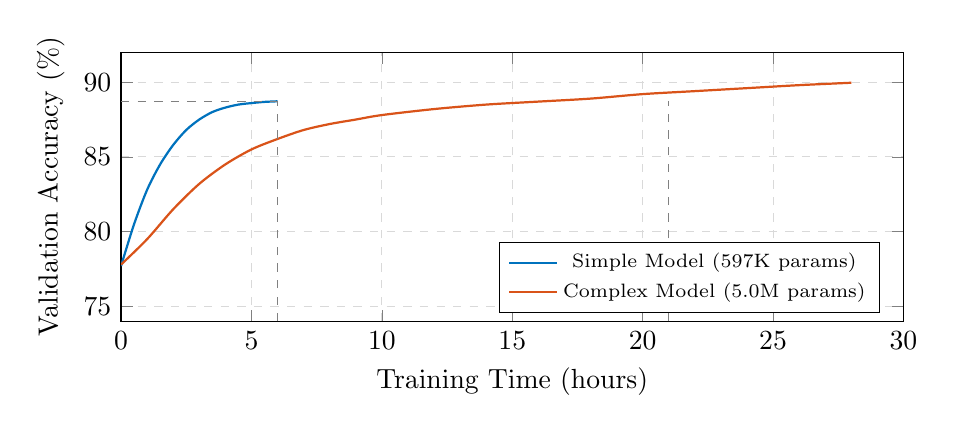
\begin{tikzpicture}
        \begin{axis}[
            width=0.95\columnwidth,
            height=5cm,
            xlabel={Training Time (hours)},
            ylabel={Validation Accuracy (\%)},
            xmin=0, xmax=30,
            ymin=74, ymax=92,
            legend pos=south east,
            legend style={font=\scriptsize},
            grid=major,
            grid style={dashed, gray!30},
        ]
        % Simple Model
        \addplot[color=matlabBlue, thick, smooth] coordinates {
            (0,77.7) (0.5,80.5) (1,82.8) (1.5,84.5) (2,85.8) (2.5,86.8) (3,87.5) (3.5,88.0) (4,88.3) (4.5,88.5) (5,88.6) (5.5,88.68) (6,88.72)
        };
        \addlegendentry{Simple Model (597K params)}
        
        % Complex Model
        \addplot[color=matlabOrange, thick, smooth] coordinates {
            (0,77.8) (1,79.5) (2,81.5) (3,83.2) (4,84.5) (5,85.5) (6,86.2) (7,86.8) (8,87.2) (9,87.5) (10,87.8) (12,88.2) (14,88.5) (16,88.7) (18,88.9) (20,89.2) (22,89.4) (24,89.6) (26,89.8) (28,89.96)
        };
        \addlegendentry{Complex Model (5.0M params)}
        
        % Reference lines
        \draw[dashed, gray] (axis cs:6,74) -- (axis cs:6,88.72);
        \draw[dashed, gray] (axis cs:0,88.72) -- (axis cs:6,88.72);
        \draw[dashed, gray] (axis cs:21,74) -- (axis cs:21,88.72);
        
        \end{axis}
    \end{tikzpicture}
    \caption{Training time comparison between simple and complex models. The complex model requires approximately 3.5$\times$ longer to reach the same accuracy as the simple model.}
    \label{fig:complexity_tradeoff}
\end{figure}

The TCR analysis in \cref{tab:tcr} reveals that the complex model requires 4-8$\times$ longer training time to achieve the same accuracy levels as the simple model.
The Learning Efficiency of the simple model (LE = 1.84\%/h) is approximately 4$\times$ higher than the complex model (LE = 0.43\%/h).

%%% Table: Time Cost Ratio
\begin{table}[t]
    \centering
    \caption{Time Cost Ratio Analysis at Different Accuracy Levels}
    \label{tab:tcr}
    \begin{tabular}{cccc}
        \toprule
        \textbf{Target Acc.} & \textbf{Simple (h)} & \textbf{Complex (h)} & \textbf{TCR} \\
        \midrule
        84\% & 1.32 & 10.28 & 7.79 \\
        86\% & 2.38 & 13.74 & 5.77 \\
        88\% & 4.34 & 18.24 & 4.21 \\
        \bottomrule
    \end{tabular}
\end{table}

These results demonstrate that for resource-constrained embedded systems, the simpler model architecture provides an optimal balance between prediction accuracy and computational efficiency.

\subsection{Impact of Window Size}

The window size significantly affects model performance, as shown in \cref{tab:window_size}.
Increasing the window size from 15 to 50 time steps improves accuracy by approximately \qty{5}{\percent}.

%%% Table: Window Size
\begin{table}[t]
    \centering
    \caption{Impact of Window Size on Model Performance}
    \label{tab:window_size}
    \begin{tabular}{ccc}
        \toprule
        \textbf{Window Size} & \textbf{Accuracy (\%)} & \textbf{RMSE} \\
        \midrule
        15 (1.5s) & 83.86 & 0.00119 \\
        50 (5.0s) & 88.72 & 0.00104 \\
        \bottomrule
    \end{tabular}
\end{table}

Larger windows capture more temporal context, enabling the model to learn longer-term dependencies in vehicle dynamics.
At 10~Hz sampling frequency, a window of 50 time steps corresponds to 5 seconds of driving data, which provides sufficient context for predicting steering torque requirements.

\subsection{Attention Weight Analysis}

\cref{fig:attention_weights} visualizes the average attention weight distributions for each mechanism.
The Simple Attention assigns progressively higher weights to more recent time steps, confirming the intuition that recent vehicle dynamics are most relevant for steering torque prediction.

%%% Figure: Attention Weights
\begin{figure}[t]
    \centering
    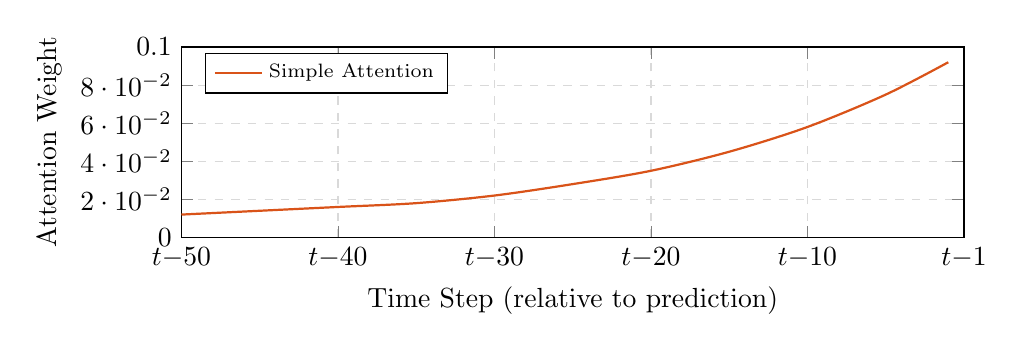
\begin{tikzpicture}
        \begin{axis}[
            width=0.95\columnwidth,
            height=4cm,
            xlabel={Time Step (relative to prediction)},
            ylabel={Attention Weight},
            xmin=-50, xmax=0,
            ymin=0, ymax=0.1,
            xtick={-50,-40,-30,-20,-10,0},
            xticklabels={$t{-}50$,$t{-}40$,$t{-}30$,$t{-}20$,$t{-}10$,$t{-}1$},
            legend pos=north west,
            legend style={font=\scriptsize},
            grid=major,
            grid style={dashed, gray!30},
        ]
        % Simple Attention weights (increasing toward recent)
        \addplot[color=matlabOrange, thick, smooth] coordinates {
            (-50,0.012) (-45,0.014) (-40,0.016) (-35,0.018) (-30,0.022) (-25,0.028) (-20,0.035) (-15,0.045) (-10,0.058) (-5,0.075) (-1,0.092)
        };
        \addlegendentry{Simple Attention}
        
        \end{axis}
    \end{tikzpicture}
    \caption{Average attention weight distribution for Simple Attention across the sliding window. Recent time steps receive higher weights, indicating their greater importance for prediction.}
    \label{fig:attention_weights}
\end{figure}

Interestingly, while Additive and Scaled Dot-Product Attention exhibit different attention patterns (the former focusing on recent steps, the latter on diagonal/adjacent steps), both achieve similar prediction performance.
This suggests that multiple attention strategies can effectively extract relevant information from the temporal sequence, but the simpler approach proves more efficient for this application.

%%%
% CONCLUSION
%%%
\section{Conclusion}
\label{sec:conclusion}

This paper presented a systematic investigation of attention-enhanced LSTM networks for steering torque prediction in Electric Power Steering systems.
Our experimental results on real-world driving data demonstrate that:

\begin{itemize}
    \item The LSTM model with Simple Attention achieves the highest prediction accuracy (\qty{89.71}{\percent}), outperforming the baseline LSTM by \qty{5}{\percent} and more complex attention mechanisms by approximately \qty{1}{\percent}.
    \item Simpler model architectures achieve comparable performance with significantly reduced computational cost, with the simple model demonstrating 4$\times$ higher learning efficiency than the complex model.
    \item Larger sliding window sizes capture more relevant temporal information, with a window of 50 time steps (5 seconds) providing optimal performance.
\end{itemize}

The proposed approach offers practical benefits for EPS system development: accurate steering torque prediction can enable proactive power management, provide safety redundancy through predictive reference values, and support the analysis of steering characteristics across different vehicle models.

Future work will explore: (1) larger window sizes with memory-efficient implementations, (2) attention mechanisms across input features rather than time steps, (3) generalization to multiple vehicle models, and (4) integration with physics-based models for improved interpretability.

\begin{thebibliography}{00}

\bibitem{isah2019electric}
A. D. Isah, A. Mohammed, and A. Hamza, ``Electric power-assisted steering: A review,'' in \textit{Proc. 2nd Int. Conf. IEEE Nigeria Computer Chapter (NigeriaComputConf)}, 2019, pp. 1--6, doi: 10.1109/NigeriaComputConf45974.2019.8949620.

\bibitem{salih2020computation}
S. Salih and R. Olawoyin, ``Computation of safety architecture for electric power steering system and compliance with ISO 26262,'' SAE Technical Paper 2020-01-0649, 2020, doi: 10.4271/2020-01-0649.

\bibitem{govender2016modelling}
V. Govender and S. M\"uller, ``Modelling and position control of an electric power steering system,'' \textit{IFAC-PapersOnLine}, vol. 49, no. 11, pp. 312--318, 2016, doi: 10.1016/j.ifacol.2016.08.047.

\bibitem{zheng2023research}
Z. Zheng and J. Wei, ``Research on active disturbance rejection control strategy of electric power steering system under extreme working conditions,'' \textit{Measurement and Control}, vol. 57, no. 1, pp. 90--100, 2023, doi: 10.1177/00202940231192986.

\bibitem{vanwijk2022data}
R. van Wijk, A. M. R. Lazcano, X. C. Akutain, and B. Shyrokau, ``Data-driven steering torque behaviour modelling with hidden Markov models,'' \textit{IFAC-PapersOnLine}, vol. 55, no. 29, pp. 31--36, 2022, doi: 10.1016/j.ifacol.2022.10.227.

\bibitem{xing2020driver}
Y. Xing, C. Lv, H. Wang, D. Cao, E. Velenis, and F.-Y. Wang, ``Driver activity recognition for intelligent vehicles: A deep learning approach,'' \textit{IEEE Trans. Veh. Technol.}, vol. 68, no. 6, pp. 5379--5390, 2019, doi: 10.1109/TVT.2019.2908425.

\bibitem{hochreiter1997long}
S. Hochreiter and J. Schmidhuber, ``Long short-term memory,'' \textit{Neural Computation}, vol. 9, no. 8, pp. 1735--1780, 1997, doi: 10.1162/neco.1997.9.8.1735.

\bibitem{gers2000learning}
F. A. Gers, J. Schmidhuber, and F. Cummins, ``Learning to forget: Continual prediction with LSTM,'' \textit{Neural Computation}, vol. 12, no. 10, pp. 2451--2471, 2000, doi: 10.1162/089976600300015015.

\bibitem{bahdanau2016neural}D. Bahdanau, K. Cho, and Y. Bengio, ``Neural machine translation by jointly learning to align and translate,'' in \textit{Proc. Int. Conf. Learn. Represent. (ICLR)}, 2015, arXiv:1409.0473.

\bibitem{vaswani2017attention}
A. Vaswani \textit{et al.}, ``Attention is all you need,'' in \textit{Proc. Adv. in Neural Inf. Process. Syst. (NeurIPS)}, 2017, pp. 5998--6008, arXiv:1706.03762.

\bibitem{govender2016pid}
V. Govender, G. Khazardi, T. Weiskircher, D. Keppler, and S. M\"uller, ``A PID and state space approach for the position control of an electric power steering,'' in \textit{Proc. 16th Int. Stuttgart Symp.}, 2016, pp. 755--769, doi: 10.1007/978-3-658-13255-2\_55.

\bibitem{marouf2011control}
A. Marouf, C. Sentouh, M. Djema\"i, and P. Pudlo, ``Control of electric power assisted steering system using sliding mode control,'' in \textit{Proc. 14th Int. IEEE Conf. Intell. Transp. Syst. (ITSC)}, 2011, pp. 107--112, doi: 10.1109/ITSC.2011.6082987.

\bibitem{lee2018robust}
D. Lee, K. Yi, S. Chang, B. Lee, and B. Jang, ``Robust steering-assist torque control of electric-power-assisted-steering systems,'' \textit{Mechatronics}, vol. 49, pp. 157--167, 2018, doi: 10.1016/j.mechatronics.2017.12.007.

\bibitem{shtessel2014sliding}
Y. Shtessel, C. Edwards, L. Fridman, and A. Levant, \textit{Sliding Mode Control and Observation}. Springer, 2013, ISBN: 978-0-8176-4893-0.

\bibitem{zhao2022modeling}
R. Zhao, W. Deng, B. Ren, and J. Ding, ``Modeling on steering feedback torque based on data-driven method,'' \textit{IEEE/ASME Trans. Mechatronics}, vol. 27, no. 5, pp. 2775--2785, 2022, doi: 10.1109/TMECH.2021.3119751.

\bibitem{wang2016financial}
J. Wang, J. Wang, W. Fang, and H. Niu, ``Financial time series prediction using Elman recurrent random neural networks,'' \textit{Comput. Intell. Neurosci.}, vol. 2016, Art. no. 4742515, 2016, doi: 10.1155/2016/4742515.

\bibitem{wan2023short}
A. Wan, Q. Chang, A. Khalil, and J. He, ``Short-term power load forecasting for combined heat and power using CNN-LSTM enhanced by attention mechanism,'' \textit{Energy}, vol. 282, Art. no. 128274, 2023, doi: 10.1016/j.energy.2023.128274.

\bibitem{li2023ultra}
K. Li, W. Huang, G. Hu, and J. Li, ``Ultra-short term power load forecasting based on CEEMDAN-SE and LSTM neural network,'' \textit{Energy Build.}, vol. 279, Art. no. 112666, 2023, doi: 10.1016/j.enbuild.2022.112666.

\bibitem{wen2023time}
X. Wen and W. Li, ``Time series prediction based on LSTM-Attention-LSTM model,'' \textit{IEEE Access}, vol. 11, pp. 48322--48331, 2023, doi: 10.1109/ACCESS.2023.3276628.

\bibitem{peng2013simulation}
J. Peng, H. He, and N. Feng, ``Simulation research on an electric vehicle chassis system based on a collaborative control system,'' \textit{Energies}, vol. 6, pp. 312-328, 2013, doi: 10.3390/en6010312.

\bibitem{commasteeringcontrol}
V. Aithan and H. Sch\"afer, ``comma-steering-control,'' GitHub, 2023. [Online]. Available: https://github.com/commaai/comma-steering-control

\bibitem{openpilot}
comma.ai, ``openpilot,'' GitHub, 2018. [Online]. Available: https://github.com/commaai/openpilot

\bibitem{kingma2015adam}
D. P. Kingma and J. Ba, ``Adam: A method for stochastic optimization,'' in \textit{Proc. Int. Conf. Learn. Represent. (ICLR)}, 2015, arXiv:1412.6980.

\bibitem{akiba2019optuna}
T. Akiba, S. Sano, T. Yanase, T. Ohta, and M. Koyama, ``Optuna: A next-generation hyperparameter optimization framework,'' in \textit{Proc. 25th ACM SIGKDD Int. Conf. Knowl. Discovery Data Mining}, 2019, pp. 2623--2631, doi: 10.1145/3292500.3330701.

\end{thebibliography}

\end{document}